\documentclass[aspectratio=169]{ISAE-Beamer}
\usefonttheme[onlymath]{serif}
\usepackage{amsmath,amssymb,amsthm}
\usepackage{bm}

\usepackage{graphicx}
\usepackage{diffcoeff}
\usepackage{dsfont}
\usepackage{mathrsfs}
\usepackage{tcolorbox}

%\usepackage{multimedia}
\usepackage{media9}
\usepackage[backend=bibtex,doi=false,isbn=false,url=false,eprint=false]{biblatex}

\graphicspath{{../images/}}

\bibliography{../mybibliography}

% Math macros
\DeclareMathOperator*{\grad}{grad}
\DeclareMathOperator*{\Grad}{Grad}
\DeclareMathOperator*{\Div}{Div}
\renewcommand{\div}{\operatorname{div}}
\DeclareMathOperator*{\Hess}{Hess}
\DeclareMathOperator*{\curl}{curl}
\DeclareMathOperator{\Tr}{Tr}
\DeclareMathOperator{\Dom}{Dom}
\DeclareMathOperator*{\esssup}{ess\,sup}

\newcommand{\bbR}{\mathbb{R}}
\newcommand{\bbF}{\mathbb{F}}
\newcommand{\bbA}{\mathbb{A}}
\newcommand{\bbB}{\mathbb{B}}
\newcommand{\bbS}{\mathbb{S}}

\newcommand*{\norm}[1]{\ensuremath{\left\|#1\right\|}}
\newcommand{\where}{\qquad \text{where} \qquad}
\newcommand{\inner}[3][]{\ensuremath{\left\langle #2, \, #3 \right\rangle_{#1}}}
\newcommand{\bilprod}[2]{\left\langle \left\langle \, #1, #2 \, \right\rangle \right\rangle}
\newcommand{\pder}[2]{\ensuremath{\partial_{#2} #1}}
\newcommand{\dder}[2]{\ensuremath{\delta_{#2} #1}}
\newcommand{\secref}[1]{\S\ref{#1}}
\newcommand{\energy}[1]{\frac{1}{2} \int_{\Omega} \left\{ #1 \right\} \d\Omega}
\newcommand{\crmat}[1]{\ensuremath{\left[#1\right]_\times}}
\newcommand{\fenics}{\textsc{FEniCS}\xspace}
\newcommand{\firedrake}{\textsc{Firedrake}\xspace}

\DeclareMathOperator*{\argmax}{arg\,max}
\DeclareMathOperator*{\argmin}{arg\,min}

\def\onedot{$\mathsurround0pt\ldotp$}
\def\cddot{% two dots stacked vertically
	\mathbin{\vcenter{\baselineskip.67ex
			\hbox{\onedot}\hbox{\onedot}}%
}}

\renewcommand\bibfont{\scriptsize}


\makeatletter \renewcommand\d[1]{\ensuremath{%
		\;\mathrm{d}#1\@ifnextchar\d{\!}{}}}
\makeatother

\title[58th CDC conference]{A port-Hamiltonian formulation of flexible structures \\
Modelling and structure preserving finite element discretization}

%\institute[ISAE]
%{\inst{1}ISAE-SUPAERO, Toulouse}

\author[Andrea Brugnoli]{Andrea Brugnoli\\
	{\and} \\
	{\textit{Supervisors}} \\
	{Daniel Alazard} \\ {Valérie Pommier-Budinger}}

\date[Toulouse, 9/11/20]{November, the 9th, 2020}

%\thanks{}

\begin{document}

\maketitle

\begin{frame}{Outline}

\tableofcontents

\end{frame}

\section{Introduction}

\begin{frame}{Twenty years of distributed port-Hamiltonian systems}
Distributed port-Hamiltonian systems were first introduced twenty years ago. \\ They have been used for simulating and controlling a variety of applications:
\begin{itemize}
	\item {flexible thin beams;}
	\item {acoustic waves;}
	\item {stirred tank reactors;}
	\item {plasma in tomahawks;}
	\item {fluid-structure interactions.}
\end{itemize}
\end{frame}

\begin{frame}{Motivation \& Research Objectives}

\begin{alertblock}{A missing piece in the port-Hamiltonian literature}
Despite all the preexisting literature, models arising from structural mechanics on multidimensional geometrical domains have rarely been considered\footfullcite{macchelli2005mindlin}. 
\end{alertblock}

\begin{block}{Purpose of this work}
This thesis tries to establish a clear connection between linear structural mechanics models
and port-Hamiltonian systems, both for the modelling and discretization tasks.
\end{block}

\begin{exampleblock}{Methodologies}
The numerical implementation relies on efficient and well-established libraries. No need to construct everything from scratch.
\end{exampleblock}

\end{frame}

\section{Port-Hamiltonian formulation of Elasticity and Thermoelasticity}

\subsection{Linear elasticity and plate models}

\begin{frame}{The Linear Elastodynamics problem}
For small deformations, the displacement within a continuum $\bm{u}$ satisfies the PDE
\begin{equation*}
\rho \diffp[2]{\bm{u}}{t} - \Div(\bm{\mathcal{D}} \Grad \bm{u}) =0, \qquad \bm{x} \in \Omega \subset \bbR^d, \; d \in \{2,3\}.
\end{equation*}
\only<1>{
\begin{itemize}
\item $\rho$ mass density;
\item $\bm{\mathcal{D}}(\cdot) = \frac{E}{1 + \nu} \left[(\cdot) + \frac{\nu}{1-2\nu}\Tr(\cdot) \bm{I} \right]$ the stiffness tensor;
\item $\Grad \bm{u} = \frac{1}{2}\left[\nabla\bm{u} + \nabla^\top\bm{u} \right]$ the symmetric gradient;
\item $\bm{\Sigma} = \bm{\mathcal{D}} \bm{\varepsilon}, \; \bm{\varepsilon} = \Grad \bm{u}$ the stress and strain tensor;
\item $\Div \bm{\Sigma} = \left(\sum_{i=1}^d \diffp{\Sigma_{ij}}{x_i}\right)_{1\le j\le d }$ the tensor divergence.
\end{itemize}
}
\only<2>{
\begin{figure}
	\centering
	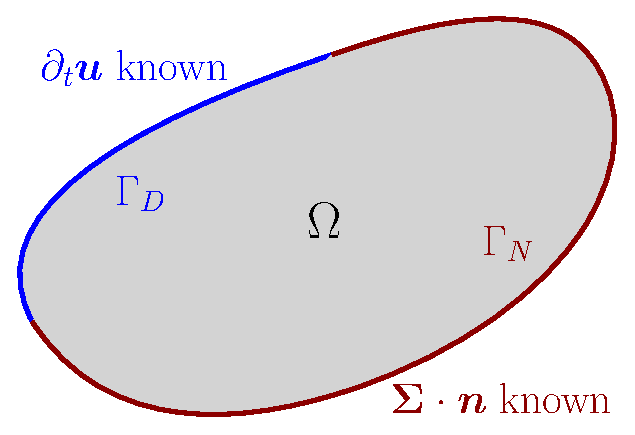
\includegraphics[height=0.5\textheight]{part_2/bc_elas2D.eps}
	\caption{A 2D continuum with Neumann and Dirichlet boundary conditions}
\end{figure}
}
\end{frame}

\begin{frame}{The port-Hamiltonian formulation}
	To derive a pH formulation, the total energy is needed
	\begin{equation*}
	H = \energy{\rho \norm{\partial_t \bm{u}}^2 + \bm{\Sigma} \cddot \bm{\varepsilon}}, \qquad \bm{A} \cddot \bm{B} \quad \text{Tensor contraction}.
	\end{equation*}
	Consider the energy variables
	\[\bm{\alpha}_v = \rho \bm{v}, \qquad \bm{A}_{\varepsilon} = \bm{\varepsilon}. \]
	The Hamiltonian is a quadratic functional in this variables
	\begin{equation*}
	H = \energy{\frac{1}{\rho} \norm{\bm{\alpha}_v}^2 + (\bm{\mathcal{D}} \bm{A}_{\varepsilon}) \cddot  \bm{A}_{\varepsilon}}.
	\end{equation*} 
\end{frame}



\begin{frame}{Structure preserving discretization}
The main properties of the dpH (conservative, passive system) are preserved at a discrete level.
\begin{columns}[T]
	\setlength{\abovedisplayskip}{1pt}
	\setlength{\belowdisplayskip}{1pt}
	\begin{column}{.4\textwidth}
		\begin{block}{Infinite dimensional pHs \only<2>{(linear case)}}
			PDE:
			\begin{align*}
			\partial_t{x}(z, t) &= \mathcal{J} \only<1>{\displaystyle \diffd{H}{x}} \only<2>{\mathcal{Q} x} + B \textcolor{red}{u(z, t)}, \\
			\textcolor{red}{y(z, t)} &= B^* \only<1>{\displaystyle \diffd{H}{x}} \only<2>{\mathcal{Q} x}.
			\end{align*}
			Boundary conditions: 
			\[\textcolor{blue}{u_\partial} = \mathcal{B} \only<1>{\displaystyle \diffd{H}{x}} \only<2>{\mathcal{Q} x}, \quad \textcolor{blue}{y_\partial} = \mathcal{C} \only<1>{\displaystyle \diffd{H}{x}} \only<2>{\mathcal{Q} x} \]
			Power balance (Stokes Theorem): 
			\[ \dot{H} = \displaystyle \int_{\partial \Omega} \textcolor{blue}{u_\partial y_\partial} \d{s} +  \int_{\Omega} \textcolor{red}{u(z, t) y(z, t)} \d{\Omega}
			\]
		\end{block}
	\end{column}
	\begin{column}{.4\textwidth}
		\begin{block}{Finite dimensional pHs \only<2>{(linear case)}}
			ODE:
			\begin{align*}
			\dot{x} &= J \only<1>{\displaystyle \partial_x {H}} \only<2>{Q x} + B_d \textcolor{red}{u_d} + B_\partial \textcolor{blue}{u_\partial}, \\
			\textcolor{red}{y_d} &= B_d^T \only<1>{\displaystyle \partial_x {H}} \only<2>{Q x}, \\
			\textcolor{blue}{y_\partial} &= B_\partial^T \only<1>{\displaystyle \partial_x {H}} \only<2>{Q x}
			\end{align*}
			Power balance: 
			\[ \dot{H} = \textcolor{blue}{u_\partial^T y_\partial} +  \textcolor{red}{u_d^T y_d}
			\]
		\end{block}
	\end{column}
\end{columns}

\end{frame}

\begin{frame}{}
\begin{exampleblock}{Available methods}
	\begin{itemize}
		\item Spectral methods (Moulla 2012):
		\begin{itemize}
			\item[\textcolor{green}{\checkmark}] Rapid spectral convergence;
			\item[\textcolor{red}{$\times$}] Only for 1D problem;
		\end{itemize}
		\item Finite differences (Trenchant 2018);
		\begin{itemize}
			\item[\textcolor{green}{\checkmark}] Valid up to 2D geometries;
			\item[\textcolor{red}{$\times$}] Requires \textit{ad hoc} implementation (staggered grids);
		\end{itemize}
		\item Finite elements based
		\begin{itemize}
			\item Golo 2004, Kotyczka 2018: the implementation requires exterior calculus knowledge and depends on the some parameters that ensure the preservation of power flow;		
			\item \textcolor{blue}{Cardoso-Ribeiro 2018}:
			\begin{itemize}
				\item[\textcolor{green}{\checkmark}] Natural extension of the mixed finite element method to pH systems;
				\item[\textcolor{green}{\checkmark}] Implementable using well-established libraries (Fenics, Firedrake);
			\end{itemize}
		\end{itemize}
	\end{itemize}
\end{exampleblock}
\end{frame}


\section{Structure preserving discretization}

\subsection{The partitioned finite element method}



\begin{frame}{The partitioned finite element method (PFEM)}
General form of a linear pH system in co-energy variables
\begin{equation*}
\mathcal{M} \diffp{e}{t} = \mathcal{J} e, \qquad \mathcal{M} = \mathcal{Q}^{-1}
\end{equation*}

\begin{block}{General procedure for PFEM}
	\setlength{\abovedisplayskip}{1pt}
	\setlength{\belowdisplayskip}{1pt}
	\begin{enumerate}
		\item Put the system into weak form:
		\begin{equation*}
		\left(v, \mathcal{M} \diffp{e}{t} \right)_{\Omega} = \left(v, \mathcal{J} e \right)_{\Omega}.
		\end{equation*}
		\item Apply integration by part on a partition of $\mathcal{J}$:
		\begin{equation*}
		\left(v, \mathcal{J} e \right)_{\Omega} \overbrace{=}^{i.b.p.} j(v, e)_{\Omega} + b(v, u_\partial)_{\partial \Omega},
		\end{equation*}
		so that $j(v, e)_{\Omega}$ is a skew-symmetric bilinear form.
		\item Discretization by Galerkin method (same basis function for test and co-energy variables)
	\end{enumerate}
\end{block}
\end{frame}



\begin{frame}{Results}
\begin{center}
	\onslide*<1>{
		\setlength{\abovedisplayskip}{0pt}
		\setlength{\belowdisplayskip}{0pt}
		Distributed load ($t_{\text{end}} = 10 \, [\mathrm{ms}]$)
		\begin{equation*}
		p = \begin{cases}
		10^5 \left[ y + 10 \left( y - L_y/2 \right)^2 \right] [Pa], \quad &\forall \, t < 2 \, [\mathrm{ms}], \\
		0, \quad &\forall \, t \ge 2 \, [\mathrm{ms}].
		\end{cases}
		\end{equation*}
		\begin{columns}
			\begin{column}{.45\textwidth}
				\includemedia[
				label=vidNoRod,
				addresource=/home/a.brugnoli/Videos_defense/Kirchh_NoRod.mp4,
				activate=pageopen,
				width=6cm, height=5cm,
				flashvars={
					source=/home/a.brugnoli/Videos_defense/Kirchh_NoRod.mp4
					&loop=true
				}
				]{}{VPlayer.swf}
			\end{column}
			\begin{column}{.45\textwidth}
				\includemedia[
				label=vidRod,
				addresource=/home/a.brugnoli/Videos_defense/Kirchh_Rod.mp4,
				activate=pageopen,
				width=6cm, height=5cm,
				flashvars={
					source=/home/a.brugnoli/Videos_defense/Kirchh_Rod.mp4
					&loop=true
				}
				]{}{VPlayer.swf}
			\end{column}
		\end{columns}
	
	\mediabutton[
	mediacommand=vidNoRod:playPause,
	mediacommand=vidRod:playPause
	]{\fbox{Play/Pause}}
				
		%\movie[width=0.8\textwidth, height=0.6\textheight]{Plate and rod}{../Videos/Comparison_RodNoRod.mp4}	
	}
	
	\end{center}
\end{frame}

\section{Stabilization by boundary injection}

\begin{frame}{Boundary stabilization of the Kirchhoff plate}
\only<1>{Consider the problem
	\begin{equation*}\small
	\begin{bmatrix}
	\rho h & 0 \\ 0 & \mathbb{D}^{-1} \\
	\end{bmatrix}
	\diffp{}{t}
	\begin{bmatrix}
	\partial_t w \\ \bm{M} \\
	\end{bmatrix} = 
	\begin{bmatrix}
	0 & -\div\Div \\ \nabla^2 & 0 \\
	\end{bmatrix}
	\begin{bmatrix}
	\partial_t w \\ \bm{M} \\
	\end{bmatrix} \quad (x, y) \in \Omega = [0, 1]\times[0,1]
	\end{equation*}
	subjected to the following boundary conditions
	\begin{align*}
	\begin{aligned}
	\partial_t w|\textcolor{blue}{\Gamma_D} &= 0, \\
	\partial_x \partial_t w|\textcolor{blue}{\Gamma_D} &= 0, \\
	\end{aligned} \qquad \textcolor{blue}{\Gamma_D} &= \left\{x = 0 \right\}\\
	\begin{aligned}
	{M}_{nn}|\textcolor{red}{\Gamma_N} &= u_M, \; \\
	\widetilde{q}|\textcolor{red}{\Gamma_N} &= u_F,\\
	\end{aligned} \qquad \textcolor{red}{\Gamma_N} &= \left\{y = 0 \cup x=1 \cup y=1 \right\}
	\end{align*}
	
	with initial conditions (compatible with the constraints):
	\[
	\partial_t w(x,y,0) = x^2; \qquad \bm{M}(x,y,0) ={0}.
	\]
}
\only<2>{ Obtain a finite-dimensional uncontrolled system
	\begin{equation*}
	\begin{aligned}
	\begin{bmatrix}
	{M} & {0} \\
	{0} & {0} \\
	\end{bmatrix}\frac{d}{d t}
	\begin{pmatrix}
	\bm{e}\\
	\bm{\lambda} \\
	\end{pmatrix}
	&= \begin{bmatrix}
	{J} & {G} \\
	-{G}^T & {0} \\
	\end{bmatrix}
	\begin{pmatrix}
	\bm{e} \\
	\bm{\lambda} \\
	\end{pmatrix} + \begin{bmatrix}
	{B} \\
	0 \\
	\end{bmatrix} \bm{u}, \\
	{y} &= \begin{bmatrix}
	{B}^T & {0} \\
	\end{bmatrix} \begin{pmatrix}
	\bm{e}\\
	\bm{\lambda} \\
	\end{pmatrix},
	\end{aligned} 
	\end{equation*}
	Apply the control law $\bm{u} = -K\bm{y}, \ K>0$
	\begin{equation*}
	\begin{bmatrix}
	M & {0} \\
	{0} & {0} \\
	\end{bmatrix}
	\frac{d}{d t}
	\begin{pmatrix}
	\bm{e}\\
	\bm{\lambda} \\
	\end{pmatrix}
	= \begin{bmatrix}
	{J} - {R} & {G} \\
	-{G}^T & {0} \\
	\end{bmatrix}
	\begin{pmatrix}
	\bm{e}\\
	\bm{\lambda} \\
	\end{pmatrix},
	\end{equation*}
	with ${R} = {B} {K} {B}^T \succeq 0$. \\
	The Hamiltonian $\dot{H} = - \bm{e}^T R \bm{e} \le 0$ is a non increasing function and by La~Salle principle the equilibrium point $\bm{e} = 0$ is asymptotically stable.	
}

\end{frame}
\begin{frame}
\begin{center}
	\only<1>{Control parameter ($t_{\text{end}} = 5 [\mathrm{s}]$)
		\begin{equation*}
		K = 
		\begin{cases}
		0, \quad &\forall t < 1 \, [\mathrm{s}], \\
		100, \quad &\forall t \ge 1 \, [\mathrm{s}].
		\end{cases}
		\end{equation*}
		\vspace{.1cm} \\
		\includemedia[
		label=vidDam,
		addresource=/home/a.brugnoli/Videos_defense/Kirchh_Damped.mp4,
		activate=pageopen,
		width=10cm, height=5cm,
		flashvars={
			source=/home/a.brugnoli/Videos_defense/Kirchh_Damped.mp4
			&loop=true
		}
		]{}{VPlayer.swf}
		
		\mediabutton[
		mediacommand=vidDam:playPause,
		]{\fbox{Play/Pause}}
		
		%\movie[width=0.42\textwidth, height = 0.7 \textheight]{Damped Kirchhoff Plate}{../Videos/Kirchh_Damped_4faster.mp4}			
	}

\end{center}
\end{frame}

\begin{frame}{Conclusion}
The following has been presented:
	\begin{itemize}
	\onslide<2->{\item the Kirchhoff plate model as a port Hamiltonian system;}
	\onslide<3->{\item a structure preserving discretization method capable of dealing with generic bcs;}
	\onslide<4->{\item interconnection with rigid elements (multibody framework);}
		\onslide<5->{\item a simple control application by damping injection;}
	\end{itemize}
	\onslide<6->{Still no rigorous proof of convergence for the finite elements. Existing solutions (only for static problems):}
	\begin{itemize}
		\onslide<7->{\item The Hellan-Herrmann-Johnson  method, but difficulties when dealing with inhomogeneous bcs;}
		\onslide<8->{\item New discretization method capable that handles inhomogeneous bcs.}
	\end{itemize}
\end{frame}


\begin{frame}{}
\centering
\Huge Thanks for your attention \\
\Huge Questions?
\end{frame}


\end{document}
